\section{Komutator i pochodna Liego}

\subsection{Komutator pól wektorowych}

\begin{lemma}
  Niech $X,Y$ będą polami wektorowymi na rozmaitości $M$. Wówczas operator 
  $$XY-YX:C^\infty(M)\to C^\infty(M)$$
  określony przez $f\mapsto XYf-YXf$ jest derywacją.
\end{lemma}

\begin{proof}
  Liniowość $XY-YX$ wynika wprost z liniowości $X$ oraz $Y$ jako operatorów na $C^\infty(M)$. Operator ten spełnia również regułę Leibniza:
  \begin{align*}
    (XY-YX)(f\cdot g)=&XY(f\cdot g)-YX(f\cdot g)=\\
    =&X(g\cdot Yf+f\cdot Yg)-Y(g\cdot Xf+f\cdot Xg)=\\
    =&X(g\cdot Yf)+X(f\cdot Yg)-Y(g\cdot Xf)-Y(f\cdot Xg)=\\
    =&{\color{blue}Yf\cdot Xg}+g\cdot XYf+{\color{orange}Yg\cdot Xf}+f\cdot XYg+\\
     &-{\color{orange}Xf\cdot Yg}-g\cdot YXf-{\color{blue}Xg\cdot Yf}-f\cdot YXg=\\
    =&g\cdot(XYf-YXf)+f\cdot(XYg-YXg)=\\
    =&g\cdot(XY-YX)f+f\cdot(XY-YX)g
  \end{align*}
\end{proof}

Lemat wyżej jest zaskakujący, gdyż np. $XY+YX$ nie jest derywacją. Jest to operator drugiego rzędu, tzn. jego wartość na funkcji $f$ zależy nie tylko of pierwszych pochodnych, ale również od pochodnych drugiego rzędu. W przypadku $XY-YX$ pochodne rzędu dwa są kasowane jak wyżej i pozostają jedynie składniki rzędu $1$.

\begin{definition}\label{komutator-definicja}
  Pole wektorowe na $M$ odpowiadające derywacji $XY-YX$ oznaczane jest symbolem $[X,Y]$ i nazywa się \important{komutatorem} pól $X$ i $Y$.

  Komutator ma następujące własności:
  \begin{multicols}{2}
  \begin{enumerate}
    \item $[X,Y]=-[Y,X]$
    \item $[[X,Y],Z]+[[Y,Z],X]+[[Z,X],Y]=0$
    \item $[X+Y,Z]=[X,Z]+[Y,Z]$
    \item $[fX,Y]=f[X,Y]-Y(f)X$
    \item $[X,fY]=Xf\cdot Y+f\cdot [X,Y]$
    \item $[cX,Y]=c[X,Y]=[X,cY]$
  \end{enumerate}
\end{multicols}
\end{definition}

\subsection{Komutator w lokalnych współrzędnych}

Niech $X=\sum X_i\frac{\partial}{\partial x_i}$ oraz $Y=\sum Y_i\frac{\partial}{\partial x_i}$ będą polami wektorowymi i $X_i,Y_i$ niech będą funkcjami współrzędnych. Wówczas:
\begin{align*}
  [X,Y]f=&XYf-YXf=\\
  =&\sum X_i\frac{\partial}{\partial x_i}\left[\sum Y_j\frac{\partial f}{\partial x_j}\right] - \sum Y_i\frac{\partial}{\partial x_i}\left[\sum X_j\frac{\partial f}{\partial x_j}\right]=\\
  =&\sum X_i\left[\sum \left[\frac{\partial Y_j\partial f}{\partial x_i\partial x_j}+Y_j\frac{\partial^2f}{\partial x_i\partial x_j}\right]\right] - \sum Y_i\left[\sum \left[\frac{\partial X_j\partial f}{\partial x_i\partial x_j}+X_j\frac{\partial^2f}{\partial x_i\partial x_j}\right]\right]=\\
  =&{\color{green}\sum_{i,j}X_iY_j\frac{\partial ^2f}{\partial x_i\partial x_j}}+\sum_{i,j}X_i\frac{\partial Y_j\partial f}{\partial x_i\partial x_j}-{\color{green}\sum_{i,j}Y_iX_j\frac{\partial^2f}{\partial x_i\partial x_j}}-\sum Y_i\frac{\partial X_j\partial f}{\partial x_i\partial x_j}=\\
  =&\sum\frac{\partial f}{\partial x_j}\left[\sum\left[X_i\frac{\partial Y_j}{\partial x_i}-Y_i\frac{\partial X_j}{\partial x_i}\right]\right]
\end{align*}
W takim razie komutator wyrażony we współrzędnych pól $X$ i $Y$ to:
$$[X,Y]=\sum\left[\sum\left[X_i\frac{\partial Y_j}{\partial x_i}-Y_i\frac{\partial X_j}{\partial x_i}\right]\right]\frac{\partial}{\partial x_j}$$

\subsection{Definicja pochodnej Liego}

%Na $\R^n$ pola wektorowe można różniczkować w różnych kierunkach, bo wektory styczne w jednym punkcie kanonicznie utożsamiają się jako wektory swobodne z wektorami stycznymi do $\R^n$ w każdym innym punkcie. Na innych rozmaitościach niekoniecznie tak jest i utożsamienia jak wyżej w różnych mapach mogą być różne.

W przestrzeni $\R^n$ możemy bez problemu zdefiniować pochodną kierunkową pola wektorowego $Y$ wzdłuż wektora $v\in T_pM$ jako
$$D_vY(p)=\frac{d}{dt}_{t=0}Y(p+tv)=\lim_{t\to0}\frac{Y(p+tv)-Y(p)}{t}$$
gdyż wektory styczne w jednym punkcie utożsamiają się jako wektory swobodne z wektorami stycznymi w każdym innym punkcie. Na innych rozmaitościach, które nie mają struktury przestrzeni wektorowej, niekoniecznie musi być to możliwe i utożsamienia takie mogą się różnić w różnych mapach.

Wzór wyżej możemy uogólniać. Pierwszą możliwością byłoby zastąpienie $Y(p+tv)$ przez krzywą całkową o początku $p$ wzdłuż wektora $Y$, ale wtedy $Y_{\gamma(t)}$ oraz $Y_{\gamma(0)}$ nie leżałyby w tej samej przestrzeni stycznej. Stąd wektor $v\in T_pM$ zastąpimy przez pole wektorowe $X$ i wektor $Y$ przesuniemy o $t$ za pomocą potoku pola $X$, po czym wrócimy je na tę samą przestrzeń w której było $Y(p)$. Działając w ten sposób definiujemy pochodną Liego.

\begin{definition}
  \important{Pochodną Liego}, $L_XY(p)$, nazywamy wektor z $T_pM$ otrzymany\marginpar{Czasem pochodną Liego w punkcie $p$ oznaczamy jako $(L_XY)_p$.} jako
  $$L_XY(p)=lim_{t\to 0}\frac{d\phi_{-t}^X[Y(\phi_t^X(p)]-Y(p)}{t}$$
  lub równoważnie
  $$\frac{d}{dt}_{t=0}d\phi_{-t}^X[Y(\phi_t^X(p))]$$
  \marginpar{$\phi_{-t}^X$ oznacza element potoku pola $X$ - górny indeks będzie informował o polu wektorowym do którego się odnosi $\phi_{-t}^X$.}
  $$\frac{d}{dt}_{t=0}(d\phi_t^X)^{-1}[Y(\phi_t^X(p)]$$
\end{definition}


  \marginpar{\Large$ $\\$ $\\\smiley{}}
\begin{illustration}
  %\draw[orange, step=0.5] (-2, -2) grid (10, 4);
  \draw[smooth cycle] plot coordinates {(-0.5, 0) (0.5, -1) (4, -1) (5, 0) (5, 1) (4.5, 1.5) (3.8, 1.5) (2.5, 0.8) (2, 0.8) (0.7, 1.5) (0, 1.5) (-0.5, 1)};
  \draw plot coordinates {(0.5, -0.5) (2, -0.5) (1.5, 0.5) (0, 0.5) (0.5, -0.5)};
  \draw plot coordinates {(2.5, -0.5) (4, -0.5) (4.5, 0.5) (3, 0.5) (2.5, -0.5)};


  \draw [smooth] plot coordinates {(-1, -1) (1, 0) (3.5, 0) (6, 1.5)};
  \filldraw (1, 0) circle (1.5pt);
  \filldraw (3.5, 0) circle (1.5pt);
  \draw[->] (3.5, 0)--(3.5, 0.8);
  \draw[->, dashed] (1, 0)--(1, 0.8);
  \draw[->] (1, 0)--(1.5, 0.8);

  \node at (1, -0.4) {$p$};
  \node at (0.8, 1) {$d\phi_{-t}^X(Y(\phi_t^X(p)))$};
  \node at (1.7, 0.5) {$Y(p)$};
  \node at (3.3, 1) {$Y(\phi_t^X(p))$};
  \node at (3.5, -0.4) {$\phi_t^X(p)$};
  
  \path[->] (3.5, -0.7) edge [bend left=40] node [midway, below] {$d\phi_{-t}^X$} (1, -0.7);
\end{illustration}

\begin{example}
  \item Rozważmy $\R^3$ jako rozmaitość i niech $X=\frac{\partial}{\partial x_1}$. Mamy wtedy
    $$\phi_t^X(x_1,x_2,x_3)=(x_1+t,x_2,x_3)$$
    $$d\phi_t^X:\underset{\scriptstyle\cong\R^3}{T_p\R^3}\to \underset{\scriptstyle\cong\R^3}{T_{\phi_t^X(p)}\R^3} = id_{\R^3}$$
    Niech teraz 
    $$Y(x_1,x_2,x_3)=\frac{\partial}{\partial x_2}+x_1\cdot\frac{\partial}{\partial x_3}$$ 
    będzie wektorem stycznym do $\R^3$ w punkcie $p=(x_1,x_2,x_3)$. Do wyliczenia pochodnej Liego potrzebujemy
    $$Y(\phi_t^X(p))=\frac{\partial}{\partial x_1}+(x_1+t)\frac{\partial}{\partial x_3}$$
    oraz
    $$(d\phi_t^X)^{-1}(Y(\phi_t^X(p)))=\frac{\partial}{\partial x_1}+(x_1+t)\frac{\partial}{\partial x_3}$$
    Skorzystamy teraz z ostatniej wariancji definicji
    $$\frac{d}{dt}_{t=0}(d\phi_t^X)^{-1}(Y(\phi_t^X(p)))=\frac{\partial}{\partial x_1}+(x_1+t)\frac{\partial}{\partial x_3}=\frac{\partial}{\partial x_3}$$
    czyli $L_X(Y)=\frac{\partial}{\partial x_3}$.
    
    \begin{center}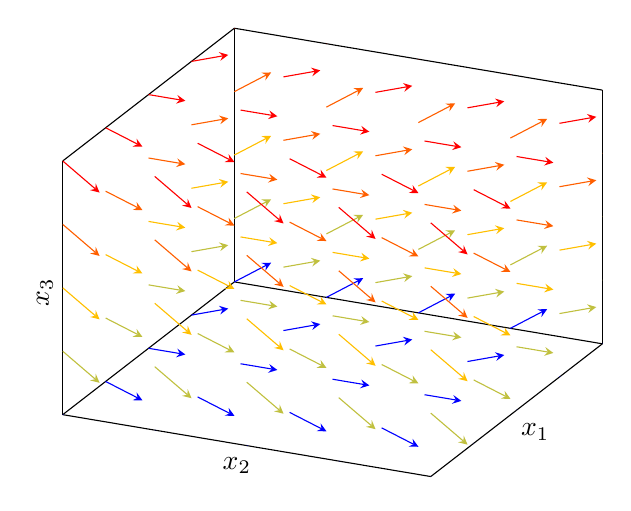
\begin{tikzpicture}
  \begin{axis}[
    domain=-1:1,
    samples=10,
    xmin=-1,xmax=1,
    ymin=-1,ymax=1,
    zmin=-1,zmax=1,
    ticks=none,
    zlabel=$x_3$,
    ylabel=$x_1$,
    xlabel=$x_2$
    ]
    \pgfplotsinvokeforeach{-1,-.5,0,.5,1}{
      \addplot3[quiver,-stealth,
        samples=5,
      %point meta={sqrt((x)^2+(y)^2+(z)^2)},
      quiver={
        u={1},
        v={0},
        w={y},
        colored, scale arrows=.2}]
      (x,y,#1);
    }
  \end{axis}
\end{tikzpicture}\end{center}

\item Rozważmy teraz $M=\R^3$ oraz pole wektorowe 
  $$X(x, y)=x\frac{\partial}{\partial y}-y\frac{\partial}{\partial x}$$
  jak w przykładzie z poprzedniego rozdziału. Wówczas 
  $$\phi_t^X(x, y)=(x\cos t-y\sin t, x\sin t+y\cos t)$$

\begin{illustration}
\begin{axis}[
    xmin = -3, xmax = 3,
    ymin = -3, ymax = 3,
    zmin = 0, zmax = 1,
    axis equal image,
    axis lines = middle,
    xtick distance = 1,
    ytick distance = 1,
    ticks = none,
    view = {0}{90},
    scale = 1.25,
    %title = {\bf Vector Field $F = [-y,x]$},
    height=7cm,
    %xlabel = {$x$},
    %ylabel = {$y$},
    colormap/viridis,
    %colorbar,
    %colorbar style = {
    %    ylabel = {Vector Length}
    %}
]
 
\addplot3[
    point meta = {sqrt(x^2+y^2)},
    quiver = {
        %u = {-y/sqrt(x^2+y^2)},
        %v = {x/sqrt(x^2+y^2)},
        u = {-y},
        v = {x},
        scale arrows = 0.4,
    },
    quiver/colored = {mapped color},
    -stealth,
    domain = -2:2,
    domain y = -2:2,
    samples=7,
    thick
] {0};
 
\end{axis}
\end{illustration}
  
$$d(\phi_t^X)_p:T_p\R^2\to T_{\phi_t^X(p)}\R^2$$
jest zadana macierzą obrotu o $t$ stopni
$$d(\phi_t^X)=\begin{bmatrix}\cos t&-\sin t\\\sin t &\cos t\end{bmatrix}$$
W takim razie macierz odwzorowania odwrotnego to
$$(d(\phi_t^X)_p)^{-1}=\begin{bmatrix}\cos t & \sin t\\-\sin t & \cos t\end{bmatrix}$$

Rozważmy teraz pole wektorowe $Y(x,y)=\frac{\partial}{\partial x}=(1, 0)$. Wtedy pochodna Liego $Y$ to
\begin{align*}
  \frac{d}{dt}_{t=0}Y(\phi_t^X(x,y))=&\frac{d}{dt}_{t=0}\begin{bmatrix}\cos t & \sin t\\-\sin t & \cos t\end{bmatrix}\begin{bmatrix}1\\0\end{bmatrix}=\\
  =&\frac{d}{dt}_{t=0}\begin{bmatrix}\cos t\\-\sin t\end{bmatrix}=\begin{bmatrix}\sin 0\\-\cos 0\end{bmatrix}=\begin{bmatrix}0\\-1\end{bmatrix}=-\frac{\partial}{\partial y}=L_X(Y)(x,y)
\end{align*}

Warto zauważyć, że $X(0,0)=0$, a jednak $L_XY(0,0)\neq 0$.
\end{example}

\subsection{Własności}

\begin{theorem}
  $$L_XY=[X,Y]$$
\end{theorem}

\begin{proof}
  Pokażemy, że dla każdego $p\in M$ $L_XY(p)=[X,Y](p)$. Rozbijemy to na przypadki w zależności od tego, czy $X(p)$ jest zerowe czy nie.

  \begin{enumerate}
    \item $\mathbf{\color{blue}X(p)\neq0}$ 

      Z \hyperref[wyprostowanie pola wektorowego]{przykładu o wyprostowywaniu pola wektorowego}\marginpar{Dla każdego pola wektorowego $X$ możemy znaleźć mapę taką, że $X=\frac{\partial}{\partial x_1}$ po wyrażeniu w tej mapie.} wiemy, że możemy dobrać mapę, w której 
      $$X(x_1,...,x_n)=\frac{\partial}{\partial x_1}$$
      oraz $p=(0,...,0)$. Niech $Y(x)=\sum_{i\leq n}Y_i(x)\frac{\partial}{\partial x_i}$ w tej mapie. Komutator $X$ i $Y$ w takim przypadku wynosi $[X,Y]=\sum\frac{\partial Y_j}{\partial x_1}(0)\cdot\frac{\partial}{\partial x_j}$, bo $X$ ma wszystkie pochodne zerowe i niezerową wartość tylko na pierwszej współrzędnej:
      \begin{align*}
        [X,Y](0)=\sum\left[\sum\left[X_i(0)\frac{\partial Y_j}{\partial x_i}(0)-Y_i(0)\frac{\partial X_j}{\partial x_i}(0)\right]\right]=\sum_{j\leq n}\frac{\partial Y_j}{\partial x_1}(0)\cdot \frac{\partial}{\partial x_j}
      \end{align*}
      
      Do wyliczenia pochodnej Liego potrzebujemy potoku pola $X$
      $$\phi_t^X(x_1,...,x_n)=(x_1+t,x_2,...,x_n)$$
      oraz jego pochodnej, czyli $d\phi_t^X=id_{\R^n}=(d\phi_t^X)^{-1}$. Podstawiając do definicji otrzymujemy
      \begin{align*}
        L_XY(0)=&\frac{d}{dt}_{t=0}(d\phi_t^X)^{-1}Y(\phi_t^X(0))=\\
        =&\frac{d}{dt}_{t=0}(d\phi_t^X)^{-1}Y(t,0,...,0)=\\
        =&\frac{d}{dt}Y(t,0,...,0)=\frac{\partial}{\partial x_1}Y(0)=[X,Y](0)
      \end{align*}
  \end{enumerate}

  Czyli po takim wyrażeniu $X$ i $Y$ w mapie mamy $[X,Y](p)=L_XY(p)$.

\item $\mathbf{\color{blue}X(p)=0}$

  Zaczniemy od udowodnienia dwóch faktów pomocniczych.

  \textbf{Fakt 1.} Jeśli $X:(a,b)\to T_pM$ oraz $f:M\to \R$ są gładkimi funkcjami, to $\frac{d}{dt}[X(t)f]=[\frac{d}{dt}X(t)]f$.

  \begin{align*}
    \frac{d}{dt}[X(t)f]=&\lim_{\varepsilon\to 0}\frac{X(t+\varepsilon)f-X(t)f}{\varepsilon}=\\
    =&\lim_{\varepsilon\to 0}\left[\frac{X(t+\varepsilon)-X(t)}{\varepsilon}\cdot f\right]\overset{\star}{=}\\
     &=\left[\lim_{\varepsilon\to0}\frac{X(t+\varepsilon)-X(t)}{\varepsilon}\right]\cdot f=\left[\frac{d}{dt}X(t)\right]f
  \end{align*}
  Równość $\star$ wynika z ciągłości pochodnej kierunkowej względem kierunku.

  \textbf{Fakt 2.} Dla $X\in C^\infty(TM)$, $f\in C^\infty(M)$ oraz dyfeomorfizmu $h:M\to N$ rozważmy pole wektorowe $dh(X)\in C^\infty(TN)$ oraz funkcję $f\circ h^{-1}\in C^\infty(N)$ przeniesione na $N$ przez $h$. Wówczas
    $$Xf(p)=dh(X)(fh^{-1})(h(p)).$$

%    \marginpar{Dowód Faktu 2. jest ćwiczeniem, tutaj }
%    Dowód pozostawiamy jako ćwiczenie.
    
%    Zgodnie z definicją podaną w 5.2 dla dowolnego $p\in M$ mamy
%    \begin{align*}
%      dh(X_{(fh^{-1})(h(p))}=&dh_{h^{-1}(fh^{-1}(h(p))}(X_{h^{-1}fh^{-1}(h(p)})=\\
%      =&dh_{h^{-1}(f(p))}(X_{h^{-1}(f(p))})
%    \end{align*}

%    Niech $X_{f(p)}=[c, t]$, wówczas $dh(X)(fh^{-1}(h(p))=dh(X)(f(h^{-1}h(p))=dh(X)f(p)=[$
%    \begin{align*}
%      [dh(X)](fh^{-1})(h(p))=&[dh(X)](h^{-1})(h(p))+h^{-1}[dh(X)]f(h(p))=\\
%      =&fdh(X)(p)+
%    \end{align*}

    Da $q\in N$ mamy\marginpar{Jak w \hyperref[przeniesione pole wektorowe]{podrozdziale 5.2 o przenoszeniu pól wektorowych przez dyfeomorfizmy.}}
    $$dh(X)=dh_{h^{-1}(q)}(X(h^{-1}(q)))$$
    ale ponieważ $h$ jest dyfeomorfizmem, to zawsze istnieje $p\in M$ takie, że $q=h(p)$. Możemy więc zapisać
    $$dh(X)=dh_{h^{-1}(h(p))}(X(h^{-1}(h(p))))=dh_p(X(p)).$$
    W takim razie
    \begin{align*}
      dh(X)(fh^{-1})(h(p))=&d_p(X(p))(fh^{-1})(h(p))=d_pX(fh^{-1}(h(p)))=d_pX(f(p))=Xf(p)
    \end{align*}
    tak jak chcieliśmy.

    Niech $f$ będzie dowolną funkcją gładką na rozmaitości $M$. Zadziałamy na nią wektorami $[X,Y](p)$ oraz $L_XY(p)$
    \begin{align*}
      [X,Y](p)f=&[X,Y]f(p)=XYf(p)-YXf(p)=-YXf(p)
    \end{align*}
    bo $X(p)=0$. Ponieważ $X(p)=0$, to na pewnym otoczeniu $p$ mamy $\phi_t^X(p)=p$ dla każdego $p$. Czyli
    \begin{align*}
      (L_XY)f(p)=&(L_XY)_pf=\left[\frac{d}{dt}_{t=0}d\phi_{-t}^X[Y(\phi_t^X(p))]\right]f=\\
      =&\left[\frac{d}{dt}_{t=0}d\phi_{-t}^X[Y(p)]\right]f\overset{F.1}{=}\frac{d}{dt}_{t=0}[d\phi_{-t}^X(Y)f(p)]\overset{F.2}{=}\\
      =&\frac{d}{dt}_{t=0}\left[Y(f\phi_{-t}^X)(\phi_t^X(p))\right]=\frac{d}{dt}[Y(f\phi_{-t}^X)(p)]=\\
      =&\frac{d}{dt}_{t=0}\frac{d}{ds}_{s=0}[f\phi_{-t}^X(\phi_s^Y(p))]=\frac{d}{ds}_{s=0}\frac{d}{dt}_{t=0}[f\phi_{-t}^X\phi_s^Y(p)]=\\
      =&\frac{d}{ds}_{s=0}-Xf(\phi_s^Y(p))=Y(-Xf(p))=-yXf(p)=[X,Y]f(p)
    \end{align*}
  
\end{proof}

Pochodna Liego ma \acc[b]{następujące własności}, które wynikają z własności komutatora:\marginpar{Własności komutatora zostały przedstawione pod \hyperref[komutator-definicja]{Definicją 6.2}}
\begin{multicols}{2}
\begin{enumerate}
  \item $L_XY=-L_YX$
  \item $L_X[Y,Z]=[L_xY,Z]+[Y,L_XZ]$ %(reguła Leibniza dla komutatora i pochodnej Liego)
  \item $L_X(Y+Z)=L_XY+L_XZ$%\columnbreak
  \item $L_{X+Y}Z=L_XY+L_YZ$
  \item $L_X(fY)=XfY+fL_XY$
  \item $L_{fX}Y=fL_XY-(Yf)X$
\end{enumerate}
\end{multicols}

\subsection{Komutowanie potoków}

\begin{definition}
  Lokalne potoki pól $X,Y$ na $M$ \important{komutują} na otoczeniu  punktu $p\in M$, jeśli istnieje $\varepsilon>0$ taki, że dla każdego $|t|,|s|<\varepsilon$ zachodzi
  \marginpar{Lee podaje $[X,Y]=0$ jako definicję komutowania potoków pól $X$ i $Y$. My podchodzimy do problemu najpierw we współrzędnych lokalnych, a dopiero potem przechodzimy do perspektywy całego $M$.}
  $$\phi_s^Y\circ\phi_t^X(q)=\phi_t^X\circ\phi_s^Y(q)$$
  dla $q$ bliskich punktowi $p$.
\end{definition}

%Oznacza to, że $YXf=XYf$ dla wszystkich $f$ gładkich na otoczeniu $p$.

\begin{theorem}
  Lokalne potoki pól $X,Y$ komutują na otoczeniu punktu $p$ $\iff$ $[X,Y]\equiv 0$ na pewnym otoczeniu punktu $p$. Oznacza to również, że $L_XY=0$ na otoczeniu punktu $p$.
\end{theorem}

\begin{proof}
  $\impliedby$

  Potrzebujemy faktu pomocniczego:

  Jeśli $\phi:M_1\to M_2$ jest dyfeomorfizmem i $X_1$ jest polem na $M_1$, a $X_2=d\phi(X_1)$ jest polem na $M_2$, to wówczas $\phi$ przenosi trajektorie pola $X_1$ na trajektorie pola $X_2$. Oznacza to, że
  $$\phi(\phi_t^{X_1}(p))=\phi_t^{X_2}(\phi(p))$$

  Zakładamy, że $L_XY=[X,Y]=0$. Możemy pokazać, że dla każdego $q\in M$ w pobliżu $p$ oraz $t_0$ bliskich $0$ mamy
  %$$0=\lim_{t\to 0}\frac{d\phi_{-t}^X[Y(\phi_t^X(p))]-Y(p)}{t}$$
  %$$0=\frac{d}{dt}_{t=0}d\phi_{-t}^X[Y(\phi_t^X(p))]$$
%
%  $$0=[X,Y]f=XYf-YXf\implies XYf=YXf$$
%  Wiemy, że $d\phi_t^X(p)=X(\phi_t^X(p))$ dla każdego $p$ oraz $t$ jako, że są to krzywe całkowe pola $X$. Czyli jeśli $X(Yf)=Y(Xf)$ dla każdego $f$, to musi być 
%  $$d\phi_t^X(Y)=Y.$$
%  W takim razie $\phi_t^X$ nałożone na trajektorie $Y$ daje nadal trajektorie $Y$, stąd potoki pola $X$ i $Y$ są względem siebie przemienne (tzn. $\phi_t^X\phi_s^Y=\phi_s^Y\phi_t^X$) i pola te komutują.
  $$\frac{d}{dt}_{t=t_0}(d\phi_{-t}^X)(Y(\phi_t^X(q))=\phi_{t_0}^X(q)$$
  To z kolei jest równe zero, bo
  \begin{align*}
    \frac{d}{dt}_{t=t_0}(d\phi_{-t}^X)(Y(\phi_t^X(q)))=&-\frac{d}{ds}_{s=0}(d\phi_{-t_0-s}^X)Y(\phi_{t_0+s}^X(q))=\\
    =&\frac{d}{ds}_{s=0}(d\phi_{-t_0}^X)(d\phi_{-s}^X)Y(\phi_s^X(\phi_{t_0}^X(q)))=\\
    =&(d\phi_{-t_0^X}\frac{d}{ds}_{s=0}(d\phi_{-s}^XY(\phi_s^X(\phi_{t_0}^X(q))=\\
    =&(d\phi_{-t_0}^X)[L_XY(\phi_{t_0}^X(q))]=\\
    =&(d\phi_{-t_0}^X)(0)=0
  \end{align*}

  Jeśli scałkujemy $L_XY$ od $0$ do $t$, dla małego $t$, to tak naprawdę całkujemy funkcję stale równą zero i dostajemy
  \begin{align*}
    0=&\int_0^{t} \frac{d}{ds}_{t=0}(d\phi_{-s}^X)(Y(\phi_s^X(q)))ds=\\
    =&(d\phi_{-t}^X)(Y(\phi_t^X(q))-(d\phi_0^X)(Y(\phi_0^X(q)))=\\
    =&(d\phi_{-t}^X)(Y(\phi_t^X(q)))-Y(q)
  \end{align*}
  bo $\phi_0^X=id$. Dla $q$ bliskich $p$ oraz małych $t$ dostajemy więc
  $$Y(q)=(d\phi_{-t}^X)(Y(\phi_t^X(q)))$$

  Zatem lokalny dyfeomorfizm $\phi_t^X$ przenosi pole $Y$ na siebie, a więc trajektorie pola $Y$ są przez niego przenoszone na trajektorie $Y$. Mamy więc
  $$\phi_t^X(\phi_s^Y(q))=\phi_s^Y(\phi_t^X(q))$$
  dla $q$ bliskich $p$ oraz małych $s$. W takim razie potoki $X$ i $Y$ komutują na otoczeniu punktu $p$.

  $\implies$

  Zauważmy najpierw, że jeśli dyfeomorfizm $\phi$ zachowuje trajektorie pola $Y$, tzn. $\phi(\phi_t^Y(q))=\phi_t^Y(\phi(q))$ dla wszystkich $q$, to pole $Y$ jest $\phi$-niezmiennicze. To znaczy $d\phi(Y)=Y$. Dokładniej mamy dla każdego $q$ $d\phi(Y(q))=Y(\phi(q))$ lub $Y(q)=(d\phi)^{-1}(Y(\phi(q)))$.

  Zakładamy, że $\phi_t^X\phi_s^Y=\phi_s^Y\phi_t^X$, czyli $\phi_t^X$ i $\phi_s^Y$ komutują wokół $p$. Wówczas dla małych $t$ $\phi_t^X$ przenosi małe kawałki trajektorii pola $Y$ w pobliżu $p$ na małe kawałki trajektorii pola $Y$. Dzięki faktowi wyżej wiemy, że wówczas
  $$(d\phi_t^X)Y(q)=Y(\phi_t^X(q)),$$
  czyli
  $$Y(q)=Y(\phi_{-t}^X(\phi_t^X(q)))=(d\phi_{-t}^X)(Y(\phi_t^X(q)))$$
  Dalsze rachunki dają
  $$L_XY(q)=\frac{d}{dt}_{t=0}(d\phi_{-t}^X)Y(\phi_t^X(q))=\frac{d}{dt}_{t=0}Y(q)=0$$
  czyli to co chcieliśmy.
\end{proof}

\subsection{Wyprostowanie komutujących pól wektorowych}

\begin{theorem} 
  Niech $X_1,...,X_k$ będą polami wektorowymi na $M$, a $dim(M)=m\geq k$. Załóżmy, że dla $q$ w otoczeniu punktu $p\in M$ pola $X_i$ 
  \begin{itemize}
    \item parami komutują oraz 
    \item są liniowo niezależne, tzn. dla $q\in M$ blisko $p$ układ $X_1(q),...,X_k(q)$ wektorów jest liniowo niezależny w $T_qM$.
  \end{itemize}

  Wówczas istnieje mapa $\phi$ wokół $p$, w której pola $X_i$ mają postać
  $$X_i(x_1,...,x_m)=\frac{\partial}{\partial x_i}$$
\end{theorem}

\begin{proof}
  Ponieważ działamy lokalnie wokół $p$, możemy przyjąć, że $M=\R^m$, $p=(0,...,0)$ oraz
  $$X_i(x)=\sum (X_i)_j(x)\cdot\frac{\partial}{\partial x_j}.$$
  Ponieważ $X_1(p),...,X_k(p)$ są liniowo niezależne, to macierz
  $$\begin{bmatrix}(X_1)_1 & (X_2)_1 & ... &\hdots (X_k)_1\\(X_1)_2 & (X_2)_2 & \hdots (X_k)_2\\
  \vdots & \vdots & \ddots & \hdots\\(X_1)_m & (X_2)_m) & \hdots & (X_k)_m\end{bmatrix}$$
  ma rząd $k$. Przyjmijmy więc, że wiersze od $1$ do $k$ tworzą macierz nieosobliwą. Możemy to zrobić, bo przenumerowanie współrzędnych nic nie psuje. Rozważmy odwzorowanie
$$\lambda(t_1,...,t_m)=\phi_{t_1}^{X_1}\circ\phi_{t_2}^{X_2}\circ...\circ\phi_{t_k}^{X_k}(0,...,0,t_{k+1},...,t_m).$$
$\lambda$ jest gładko określone na pewnym otoczeniu $(0,...,0)$ oraz
$$\lambda(0,...,0)=(0,...,0)=p.$$

Gdy $k=2$, a $m=3$, to $\lambda(x,y,z)=\phi_x^{X_1}\phi_y^{X_2}(0,0,z)$, z drugiej strony mamy równość
$$\phi_x^{X_1}\phi_y^{X_2}(0,0,z)=\phi_y^{X_2}\phi_x^{X_1}(0,0,z)$$
która wynika z rysunku

\begin{illustration}
  \draw[->] (0,0)--(0, 2);
  \draw[->] (0,0)--(3,0);
  \draw[->] (0,0)--(-0.75, -1);

  \filldraw[color=white, pattern color=green!60, pattern=crosshatch] (-0.5, 1.2)--(2.5, 1.95)--(3.25, 0)--(0.25, -0.75)--cycle;
    
\filldraw (0, 1) circle (1.5pt);
\filldraw (2, 1.5) circle (1.5pt);
\filldraw (2.5,0.2) circle (1.5pt);
\filldraw (0.5, -0.3) circle (1.5pt);

  \draw plot coordinates {(0, 1) (2, 1.5) (2.5, 0.2) (0.5, -0.3) (0, 1)};
  \draw[->](0, 1)--(1, 1.25);
  \draw[->](2, 1.5)--(2.25, 0.85);
  \draw[->] (2.5, 0.2)--(1.5, -0.05);
  \draw[->] (0.5, -0.3)--(0.25, 0.35);

  \node at (-0.5, 1) {$(0,0,z)$};
  \node at (2.3, 1.8) {$\phi_y^{X_2}(0,0,z)$};
  \node at (3.5, -0.2) {$\phi_y^{X_2}\phi_x^{X_1}(0,0,z)=\phi_x^{X_1}\phi_y^{X_2}(0,0,z)$};
  \node at (0.5, -0.6) {$\phi_x^{X_1}(0,0,z)$};
\end{illustration}

Obliczmy pochodną $\frac{\partial \lambda(t_1,...,t_m)}{\partial t_i}$ dla $i=1,...,k$
\begin{align*}
  \frac{\partial \lambda(t_1,...,t_m)}{\partial t_i}=&\frac{d}{ds}_{s=0}\phi_{t_1}^{X_1}\circ...\circ\phi_{t_i+s}^{X_i}\circ...\circ\phi_{t_k}^{X_k}(0,...,0,t_{k+1},...,t_m)=\\
  =&\frac{d}{ds}_{s=0}\phi_{t_i+s}^{X_i}\circ\phi_{t_i}^{X_1}\circ...\circ\phi_{t_k}^{X_k}(0,...,0,t_{k+1},...,t_m)=\\
  =&\frac{d}{ds}_{s=0}\phi_s^{X_i}(\phi_{t_1}^{X_1}\circ...\circ\phi_{t_i}^{X_i}\circ...\circ\phi_{t_k}^{X_k}(0,...,0,t_{k+1},...,t_m))=\\
  =&\frac{d}{ds}_{s=0}\phi_s^{X_i}(\lambda(t_1,...,t_m))=\\
  =&X_i(\lambda(t_1,...,t_m))
\end{align*}
Ponieważ $\lambda(0,...,0,t_{k+1},...,t_m)=(0,...,0,t_{k+1},...,t_m)$, to $D\lambda(0)$ zapisuje się jako macierz
$$D\lambda(0)=
\left[
  \begin{array}{c | c}
    \begin{array}{c c c}
      (X_1)_1 &\hdots & (X_k)_1\\
      \vdots & \ddots & \vdots \\ %& & & \makebox(0,0){\text{\huge0}}\\
      (X_1)_k & \hdots & (X_k)_k\\
          %& & & 1\\
      \vdots & \ddots & \vdots \\ % & 0 & 1 \\
         %& & & 0 & 0& 1\\
        (X_1)_m & \hdots & (X_k)_m %& 0 & 0 & \hdots & 1
  \end{array} & 
    \begin{array}{c}
        \makebox(0,0){\text{\huge0}}\\
          \\
          \\
      \hline
      \\
      \begin{array}{c c c c}
        1\\
        0 & 1\\
        0 & 0 & \hdots & 1
      \end{array}
    \end{array}
  \end{array}
\right]
$$
Łatwo zobaczyć, że $D\lambda(0)$ jest macierzą nieosobliwą, więc $\lambda$ jest dyfeomorfizmem na otoczeniu $0$. Ponieważ 
$$d\lambda(\frac{\partial}{\partial t_i}(t_1,...,t_m))=X_i(\lambda(t_1,...,t_m),$$
to dla mapy $\phi=\lambda^{-1}$ mamy
$$d\phi(X_i(\lambda(t_1,...,t_m))=\frac{\partial}{\partial t_i}(t_1,...,t_m)$$
czyli $X_i=\frac{\partial}{\partial t_i}$ w tej mapie.
\end{proof}
